\documentclass[11pt]{article}

\author{wilricknl}
\title{3D Math Primer - Solutions chapter 11}

\usepackage{amsmath}
\usepackage{amssymb}
\usepackage{float}
\usepackage{enumerate}
\usepackage{graphicx}
\usepackage{url}

\begin{document}

\maketitle

\section{Solutions chapter 11}

\subsection{Exercise 1}

$$\frac{1\text{lb}}{\text{in}^2} \times \frac{4.448\text{N}}{1\text{lb}} \times \left(\frac{\text{in}}{0.0254\text{m}}\right)^2=\frac{4.448\text{N}}{(0.0254\text{m})^2} = \frac{6894.4\text{N}}{\text{m}^2}$$

\subsection{Exercise 2}

\begin{figure}[H]
\centering
    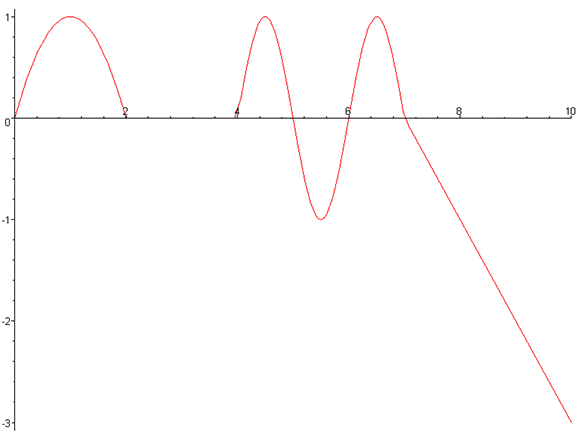
\includegraphics[width=0.6\textwidth]{exercise02}
\caption{Graph of velocity}
\label{fig:velocity-graph}
\end{figure}

\subsection{Exercise 3}

\begin{enumerate}[a.]
	\item $\frac{x(1)-x(0)}{1-1} = 1$
	\item $\frac{x(2)-x(1)}{2-1} = -1$
	\item $\frac{x(2)-x(0)}{2-0} = 0$
	\item $\frac{x(6.5)-x(5.5)}{6.5-5.5} = 2$
	\item $\frac{x(9)-x(0)}{9-0} = \frac{2}{9}$
\end{enumerate}

\subsection{Exercise 4}

\begin{equation*}
	v(t) =
	\begin{cases}
		2-2t & 0 < t < 2 \\
		0 & 2 < t < 4 \\
		\pi \cos(\pi t) & 4 < t < 7 \\
		-1 & 7 < t
	\end{cases}
\end{equation*}

\subsection{Exercise 5}

\begin{enumerate}[a.]
	\item $2-2 \cdot{} 0.1 = 1.8$
	\item $2-2 = 0$
	\item $2-3.8 = -1.8$
	\item $\pi \cdot \cos(4.1\pi) = 2.98 \dots $
	\item $\pi \cdot \cos(5\pi) = \pi$
	\item $\pi \cdot \cos(6.5\pi) = 0$
	\item $-1$
	\item $-1$
\end{enumerate}

\end{document}
